\chapter{Proposed Translator}
\label{ch:proposed-system}
As a solution to the previous chapter, this one focuses on proposing a application $f : SC' \rightarrow MO$ such that applied on a
schema, defined in \cref{eq:schema-reduction}, results in a domain model (\cref{eq:plain-object-model}) based on plain objects (\cref{eq:plain-object}).
Therefore the aim of this chapter is to once defined an schema as \cref{eq:schema-reduction} and a shape as \cref{eq:shape-reduction} define
an application $f$ such that

\begin{equation}
f(SC')=
\begin{bmatrix}f'(S'_1)
\\ f'(S'_2)
\\ \vdots
\\ f'(S'_n)
\end{bmatrix},
\end{equation}

where,

\begin{equation}
	f'(p_{SC'},t_{SC'},c_{SC'}) = (p_{S'},t_{S'}),
\end{equation}

and give a proposition for $f'(x')$ and therefore for $f(x)$.

We know that \cref{eq:shape-reduction} has been obtained in such a way that $\forall\ s' \in S'\ \exists\ f:S' \rightarrow PO$ and also in \cref{eq:values-mapping} we set
the aggregation criterion of the cardinality component over the type component to be able to create the images of $SC'$ in $MO$. Therefore $f'$ is defined as,

\begin{equation}\label{eq:transformation-f}
f':S' \rightarrow PO = f'(p_{S'},t_{S'},c_{S'}) \begin{cases}
	(p_{S'},\ Proy_{t_{S'}}lst) & if \; c_{S'}=(1,1) \\
	(p_{S'},\ List[Proy_{t_{S'}}lst]) & if \; c_{S'}=(0,\infty)
   \end{cases}
\end{equation}

where $Proy_{t_{S'}}lst$ represents the projection of the compatible type $t_{S'}$ from the shapes space of types
over the Language Specific Types space $(lst)$.

Therefore we not only know that it is possible to create a transformation from the subset of selected schemas
towards domain models formed by flat objects, but we have also identified the function that allows us to carry
out this transformation. So, next we will focus on giving shape to this function so that a system can be
implemented that performs the described transformations automatically.For this, in this section we will see
the structure of the proposed solution as well as an implementation that allows us to validate the proposed
solution to later analyze the objects generated by the solution.

\section{Structure}
Our solution is based on a code translator. In the end, a translator is still a type of compiler \cref{fig:compiler-stages},
where we have the analysis and synthesis phase. The analysis phase focuses on verifying that the input is correct and on
making the necessary transformations. While the synthesis starts from a high quality structure and performs the
appropriate transformations to reach the target representation. In the case of our solution we have a difference
and that is that we do not have a single target but multiple ones (\cref{fig:translator}).

In addition to this, in \cref{ch:proposed-sintactic-semantic-analyzer}, we have already developed a system capable of analyzing,
validating and transforming source code so that we obtained an intermediate language made up of a
high-quality graph. Therefore in our translator we will reuse the lexical, syntactic and semantic
analyzer from \cref{ch:proposed-sintactic-semantic-analyzer}, that makes the front end of our translator.
And thenm, what we will truly develop in this section, is the back-end of the translator.

\begin{figure}
    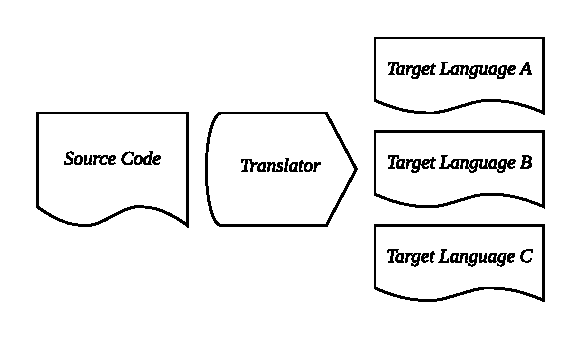
\includegraphics{images/translator.pdf}
    \centering
	\caption[Translator generic structure]{Translator generic structure.}
    \label{fig:translator}
\end{figure}

\subsection{Translator Back-end}
In our solution, the back-end of the translator, also called the synthesis phase,
fulfills two main functions. On one hand, it analyzes the intermediate language
in search of some specific incompatibility with the target language. And on the
other hand, it generates the specific code for the target language.

To perform the analysis of the intermediate language and through the Visitor pattern,
a graph path is implemented that validates that no node or set of nodes
violate the restrictions obtained in \cref{eq:schema-reduction}. The visitor that is implemented is
completely reused from the one developed for the Syntax or Semantic analysis in \cref{ch:proposed-sintactic-semantic-analyzer}.

For code generation, it is proposed to carry out an implementation of the Visitor pattern for each of the specific code generators,
each one of the specific implementations will perform the transformation function described in \cref{eq:transformation-f},
without prejudice to the fact that each specific code generator may have more implementations of the visitor associated.
\cref{fig:class-diagram-cg} illustrates this situation where the Java code generartion visitor actually contains four more visitors
one for each language specific level of the plain objects.

\begin{figure}
    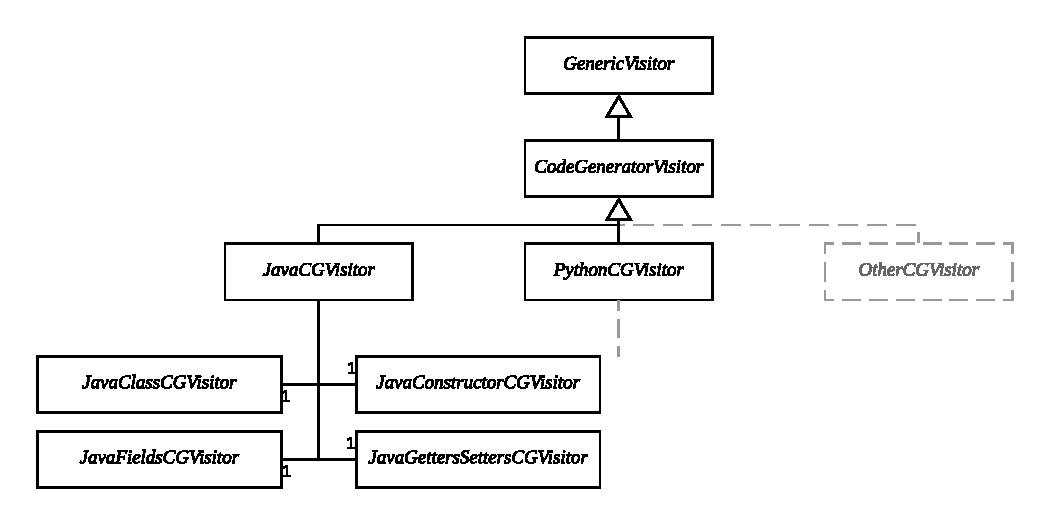
\includegraphics[width=\textwidth]{images/class-diagra-cg.pdf}
    \centering
	\caption[Class diagram example of the code generation visitors]{Class diagram example of the code generation visitors.}
    \label{fig:class-diagram-cg}
\end{figure}

And as proof of concept of the structure proposed in the previous section, we implemented a system that starts from the one
developed in \cref{sec:anal-implementation} and is capable of generating code from schematics, checking that they are valid.
This solution follows structructure developed in this system and more precisely \cref{fig:class-diagram-cg}. Moreover this
developed system offers a CLI tool (\cref{fig:menu-tool}). In this tool the users can define multiple options as \texttt{--java-pkg=STRING} which if
present will trigger the java code generation and will generate the target object in the specified package.

For example, for the input \texttt{java -jar shexlc.jar --java-pkg=demo person.shexl} where the \texttt{person.shexl}
file corresponds to the schema defined at \cref{fig:shex-translate-small} \texttt{ShEx-Lite} would generate a single java
class with the code that appears at the \texttt{Person.java} file, also in \cref{fig:shex-translate-small}.

\begin{figure}
    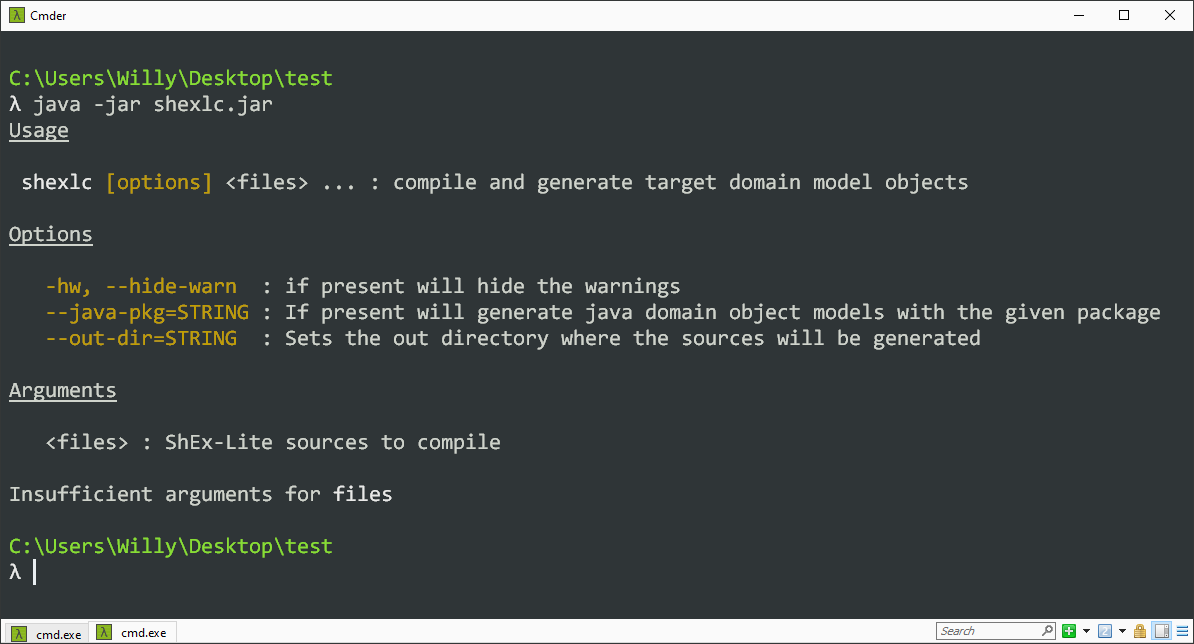
\includegraphics[width=\textwidth]{images/shexlc-menu.PNG}
    \centering
	\caption[CLI menu of \texttt{ShEx-Lite} CLI tool]{CLI menu of \texttt{ShEx-Lite} CLI tool.}
    \label{fig:menu-tool}
\end{figure}

This system
will be used for evaluating the proposed solution.

\section{Generated Obejcts}
In this section we will give real examples of use cases in which the proposed system has been used to generate objects,
in addition we will study the objects in order to estimate their quality.

\subsection{Real (Hércules ASIO European Project)}
In the framework of the European project Hercules ASIO, financed with FIVE MILLION FOUR HUNDRED SIXTY-TWO THOUSAND SIX HUNDRED
euros, the system described is used to link two parts of the architecture, the ontological infrastructure and the semantic 
infrastructure. The Hercules project tries to find a solution based on linked data to manage the research framework
in Spanish universities. Some examples of the obejects generated in this project are \cref{fig:example-2} and \cref{fig:example-3}.

\begin{center}
	\noindent\begin{minipage}[t]{.4\textwidth}
		\begin{lstlisting}[frame=topline,numbers=left,firstnumber=0,title=\scriptsize\texttt{University.shexl}, basicstyle=\ttfamily\scriptsize]{a}
# Prefixes...
asio:University {
  rdfs:name xsd:string ;
  rdfs:county   xsd:string ;
  rdfs:location xsd:String ;
  asio:hasRector
    @asio:UniversityStaff ;
	...
}
		\end{lstlisting}
	\end{minipage}\hfill
	\begin{minipage}[t]{.5\textwidth}
		\begin{lstlisting}[language=Java, frame=t,numbers=left,firstnumber=0,title=\scriptsize\texttt{University.java}, basicstyle=\ttfamily\scriptsize]{b}
// Imports...
public class University {
  private String name ;
  private String country ;
  private String location ;
  private asio.UniversityStaff hasRector ;
  ...
  // Constructor...
  // Getters and Setters...
}
		\end{lstlisting}
	\end{minipage}
	\captionof{figure}{Schema modeling a \texttt{University} in \texttt{shexl} syntax to the left. And the \texttt{ShEx-Lite} generated code in \texttt{Java} to the right.}
	\label{fig:example-2}
\end{center}

\begin{center}
	\noindent\begin{minipage}[t]{.4\textwidth}
		\begin{lstlisting}[frame=topline,numbers=left,firstnumber=0,title=\scriptsize\texttt{Researcher.shexl}, basicstyle=\ttfamily\scriptsize]{a}
# Prefixes...
asio:Researcher {
  rdfs:name xsd:string ;
  rdfs:surname   xsd:string ;
  rdfs:id xsd:integer ;
  rdfs:orcid xsd:string ;
  rdfs:publications
    @asio:AcademicPublication * ;
	...
}
		\end{lstlisting}
	\end{minipage}\hfill
	\begin{minipage}[t]{.5\textwidth}
		\begin{lstlisting}[language=Java, frame=t,firstnumber=0,numbers=left,title=\scriptsize\texttt{Researcher.java}, basicstyle=\ttfamily\scriptsize]{b}
// Imports...
public class University {
  private String name ;
  private String surname ;
  private int id ;
  private String orcid ;
  private List<asio.AcademicPublication>
    publications ;
  ...
  // Constructor...
  // Getters and Setters...
}
		\end{lstlisting}
	\end{minipage}
	\captionof{figure}{Schema modeling a \texttt{Researcher} in \texttt{shexl} syntax to the left. And the \texttt{ShEx-Lite} generated code in \texttt{Java} to the right.}
	\label{fig:example-3}
\end{center}

\subsection{Synthetic (Generated)}
In addition to the actual use case mentioned above, different generations of synthetically generated objects have been made to validate that the generation is correct.
\cref{fig:example-4} illustrates a generated schema that contains all the possible types that our solution can represent in any object oriented language.

\begin{center}
	\noindent\begin{minipage}[t]{.4\textwidth}
		\begin{lstlisting}[frame=topline,numbers=left,firstnumber=0,title=\scriptsize\texttt{Synthetic.shexl}, basicstyle=\ttfamily\scriptsize]{a}
# Prefixes...
a:b {
	:c xsd:string ;
	:d xsd:integer ;
	:e xsd:float ;
	:e xsd:boolean ;
	:f @a:b ;
}
		\end{lstlisting}
	\end{minipage}\hfill
	\begin{minipage}[t]{.5\textwidth}
		\begin{lstlisting}[language=Java, frame=t,numbers=left,firstnumber=0,title=\scriptsize\texttt{Synthetic.java}, basicstyle=\ttfamily\scriptsize]{b}
package a;
// Imports...
public class B {
	private String c;
	private int d;
	private int e;
	private a.B f;
	// Constructor...
	// Getters and Setters...
}
		\end{lstlisting}
	\end{minipage}
	\captionof{figure}{Synthetic schema in \texttt{shexl} syntax to the left. And the \texttt{ShEx-Lite} generated code in \texttt{Java} to the right.}
	\label{fig:example-4}
\end{center}